\documentclass[12pt,a4paper]{article}
\usepackage[utf8]{inputenc}
\usepackage[english]{babel} 
\usepackage{fullpage} 
\usepackage{amsmath} 
\usepackage{amsfonts} 
\usepackage{amssymb} 
\usepackage{verbatim} 
%\usepackage{listings} 
\usepackage{color} 
\usepackage{setspace} 
\usepackage{epstopdf} 
\usepackage{braket}
\usepackage{graphicx} 
\usepackage{float}
\usepackage{cite} 
\usepackage{url}
\usepackage[makeroom]{cancel}
\usepackage{caption}
\usepackage{subcaption}

\usepackage{algorithmicx}
\usepackage{algorithm}% http://ctan.org/pkg/algorithms
\usepackage{algpseudocode}% http://ctan.org/pkg/algorithmicx

\usepackage{hyperref}


\pagestyle{empty}
\usepackage[procnames]{listings}
\bibliographystyle{plain}

\makeatletter
\newcommand*{\rom}[1]{\expandafter\@slowromancap\romannumeral #1@}
\makeatother

\newcommand{\s}{^{*}}
\newcommand{\V}[1]{\textbf{#1}}
\newcommand{\husk}[1]{\color{red} #1 \color{black}}
\newcommand{\E}[1]{\cdot 10^{#1}}
\newcommand{\e}[1]{\ \text{#1}}
\newcommand{\tom}[1]{\big( #1 \big)}
\newcommand{\Tom}[1]{\Big( #1 \Big)}
\newcommand{\tomH}[1]{\big[ #1 \big] }
\newcommand{\TomH}[1]{\Big[ #1 \Big]}
\newcommand{\tomK}[1]{ \{ #1 \} }
\newcommand{\TomK}[1]{\Big\lbrace #1 \Big\rbrace}
\newcommand{\bigabs}[1]{\left| #1 \right|}

% Some commands etc. added by Simen
%\usepackage{physics}
\usepackage{units}
\newcommand\smat[1]{\big(\begin{smallmatrix}#1\end{smallmatrix}\big)}
\newcommand\ppmat[1]{\begin{pmatrix}#1\end{pmatrix}}
\newcommand\numberthis{\addtocounter{equation}{1}\tag{\theequation}}
% Usage: \numberthis \label{name}
% Referencing: \eqref{name}


\author{Eirik Ramsli Hauge}
\title{Project 1 in FYS4150}

\begin{document}
	\maketitle
	
\begin{abstract}
The aim of this numerical experiment is to solve the one-dimensional Poisson equation with Dirichlet boundary conditions. At first we will use the formula $\V{A} \V{v} = \V{p}$ and the fact that A is a tridiagnoal matrix to devlope an algorithm that we then can compare to more general methods. We found that a specialized algorithm is better than a general and that using LU-decomposition is the slowest method. The relative error of the approximation compared to the exact solution is best at $\log_{10}(h) = -5$ where $h$ is the step length.
\end{abstract}
\subsection*{Introduction}
This projects\husk{REF!} goal is to learn the students that giving a computer less things to do, makes it do the things you want it to do faster. 
\subsection*{Theory}
In this project we want to look closer at the one-dimensional Poisson's equation given as:
\begin{equation}
\frac{1}{r^2} \frac{\partial}{\partial r} \Tom{r^2 \frac{\partial \Phi}{\partial r}} = - 4 \pi \rho(r)
\label{eq:PO}
\end{equation}
where $\Phi$ is the electrostatic potential generated bya localized charge distribution $\rho(r)$. If we now do the substitution $\Phi(r) = \frac{\phi(r)}{r}$, we can rewrite equation \eqref{eq:PO} as follows:
\begin{align*}
\frac{\partial \phi}{\partial r^2} = - 4 \pi r \rho(r)
\end{align*}
By letting $\phi \rightarrow u$ and $r \rightarrow x$ we end up with:
\begin{equation}
-u^{''}(x) = f(x), \quad x \in (0,1), \quad u(0) = u(1) = 0
\label{eq:po}
\end{equation}
If we define the discretized approximation to $u$ as $v_i$, the second derivative of u can be approximated with:
\begin{align*}
- \frac{v_{i + 1} + v_{i-1} - 2v_i}{h^2} = f_i \qquad \text{for i = 1,...,n}
\end{align*}
Where $x_i = ih$ are grid points in the interval $x_0 = 0$ to $x_{n+1} = 1$ with step length $h = 1/(n+1)$ and $f_i = f(x_i)$. With the boundary conditions $v_0 = v_{n + 1} = 0$ we can see that for i = 0 we get:
\begin{align*}
-v_1 + 2v_0 &= f_0 h^2
\intertext{For i = 1:}
- v_2 -v_0 + 2v_1 &= f_1 h^2
\intertext{For i = 2}
- v_3 -v_1 + 2v_2 &= f_2 h^2
\intertext{We can easily see that this gives us:}&
\underbrace{
\begin{pmatrix}
2 & -1 & 0 & 0 & 0 & \cdots &  0 \\
-1 & 2 & -1 & 0 & 0 & \cdots & 0 \\
0 & -1 & 2 & -1 & 0 & \cdots & 0 \\
\vdots & \vdots & \vdots & \ddots & \vdots & \vdots & \vdots \\
0 & \cdots & 0 & -1 & 2 & -1 & 0 \\
0 & \cdots & 0 & 0 & -1 & 2 & -1 \\
0 & \cdots & 0 & 0 & 0 & -1 & 2  \\
\end{pmatrix}}_{\V{A}}
\underbrace{
\begin{pmatrix}
v_1 \\ v_2 \\ v_3 \\ \vdots \\ \vdots \\ \vdots \\ v_n
\end{pmatrix}}_{\V{v}} = 
\underbrace{
\begin{pmatrix}
f_1 h^2 \\ f_2 h^2 \\ f_3 h^2 \\ \vdots \\ \vdots \\ \vdots \\ f_n h^2
\end{pmatrix}}_{p}
\end{align*}
By setting $f_i h^2 = p_i$ we can write this as:
\begin{align*}
\V{A}\cdot \V{v} &= \V{p} \\
\intertext{The task \husk{Referanse} asks us to make a general algorithm to solve this scenario for any values in the tridiagonal matrix. Assuming a general tridiagonal 4x4-matrix $\widetilde{\V{A}}$ for simplicity we can illustrate the method for finding $v$ as follows:}
\begin{pmatrix}
b_1 & c_1 & 0 & 0 \\
a_2 & b_2 & c_2 & 0 \\
0 & a_3 & b_3 & c_3 \\
0 & 0 & a_4 & b_4 \\
\end{pmatrix}
\begin{pmatrix}
v_1 \\ v_2 \\ v_3 \\ v_4
\end{pmatrix} &= 
\begin{pmatrix}
p_1 \\ p_2 \\ p_3 \\ p_4
\end{pmatrix}
\end{align*}
\begin{align*}
\intertext{This gives us the following equations:}
\text{\rom{1}}:& \, v_1b_1 + c_1v_2 &= p_1 \\
\text{\rom{2}}:& \, a_2v_1 + b_2v_2 + c_2v_3 &= p_2 \\
\text{\rom{3}}:& \, a_3v_2 + b_3v_3 + c_3v_4 &= p_3 \\
\text{\rom{4}}:& \, a_4v_3 + b_4v_4 &= p4 \\
\end{align*}
We want only zeroes on the left side of the diagonal:
\begin{align*}
p_2\s &= p_2 - p_1\cdot \frac{a_2}{b_1} \\
&= a_2v_1 + b_2v_2 + c_2v_3 - v_1a_2 - v_2\frac{c_1a_2}{b_1} \\
&= v_2(b_2 - \frac{c_1a_2}{b_1}) +c_2v_3 \\
&= v_2b_2\s + c_2v_3 \\
\intertext{Now we have the following matrix:}
&\begin{pmatrix}
b_1 & c_1 & 0 & 0 \\
0 & b_2\s & c_2 & 0 \\
0 & a_2 & b_3 & c_3 \\
0 & 0 & a_3 & b_4 \\
\end{pmatrix}
\intertext{As we can see, the $a_2$-term disappers from the second row. Following this trail of thought we do the same for the next row.}
p_3\s &= p_3 - p_2\* \cdot \frac{a_3}{b_2\s} \\
&= v_3(b_3 - \frac{c_2a_3}{b_2\s}) + c_3v_4 \\
&= v_3b_3\s + c_3v_3
\end{align*}
This gives us the general idea and we can write a general expression for both $p_i\s$ and $b_i\s$:
\begin{equation}
p_i\s = p_i - p_{i-1}\frac{a_{i}}{b_{i-1}\s}, \quad \text{for i = 2,...,n}, \quad \text{and } p_1\s = p_1
\label{eq:p}
\end{equation}
\begin{equation}
b_i\s = b_i - \frac{c_{i-1}a_{i}}{b_{i-1}\s}, \quad \text{for i = 2,...,n}, \quad \text{and } b_1\s = b_1
\label{eq:b}
\end{equation}
Using equations \eqref{eq:b} and \eqref{eq:p} through the whole matrix is called forward substitution and we end up with:
\begin{align*}
\begin{pmatrix}
b_1 & c_1 & 0 & 0 \\
0 & b_2\s & c_2 & 0 \\
0 & 0 & b_3\s & c_3 \\
0 & 0 & 0 & b_4\s \\
\end{pmatrix}
\begin{pmatrix}
v_1 \\ v_2 \\ v_3 \\ v_4
\end{pmatrix}
&= \begin{pmatrix}
p_1 \\ p_2\s \\ p_3\s \\ p_4\s
\end{pmatrix}
\intertext{We want to find an expression for $v_i$ and from the last row we can find a simple equation for $v_4$}
b_4\s v_4 = p_4\s \Rightarrow v_4 &= \frac{p_4\s}{b_4\s} 
\intertext{From the second last row we find an expression for $v_3$}
b_3\s v_3 + c_3 v_4 = p_3\s \Rightarrow v_3 &= \frac{p_3\s - c_3v_4}{b_3\s}
\intertext{Again, doing this for the next row (going downward and up) we find that $v_i$ can be expressend in a general way as:}
\end{align*}
\begin{equation}
v_i = \frac{p_i\s - c_i v_{i+1}}{b_i\s}, \quad \text{for i = n-1,...,1}, \quad \text{and } v_n = \frac{p_n\s}{b_n\s}
\label{eq:v}
\end{equation}
This is called backwards substitution. \\
However, since matrix $\V{A}$ has the same values for a, b and c for all $i$, we can specialize equations \eqref{eq:p}, \eqref{eq:b} and \eqref{eq:v}. By inserting $a_i = c_i = -1$ and $b_i = 2$ in \eqref{eq:b} we can easily see that:
\begin{equation}
b_i\s = \frac{i+1}{i}, \quad \text{for i = 2,...,n}, \quad \text{and } b_1\s = b_1 = 2
\label{eq:1bs}
\end{equation}
\begin{equation}
p_i\s = p_i + \frac{p_{i-1}\s}{b_{i-1}\s}, \quad \text{for i = 2,...,n}, \quad \text{and } p_1\s = p_1
\label{eq:1ps}
\end{equation}
\begin{equation}
v_i = \frac{p_i\s + v_{i+1}}{b_i\s}, \quad \text{for i = n-1,...,1}, \quad \text{and } v_n = \frac{p_n\s}{b_n\s}
\label{eq:1vs}
\end{equation}
Since our $v_i$ is an approximation to the known solution $u_i$ we can find the relative error by:
\begin{equation}
\epsilon_i = \log_{10}\Tom{\bigabs{\frac{v_i - u_i}{u_i}}}
\label{eq:error}
\end{equation}
where the known solution $u_i$ is given as:
\begin{equation}
u_i = u(x) = 1 - (1 - e^{-10})x - e^{-10x}
\label{eq:ux}
\end{equation}
\subsubsection*{LU-decompostion}
Another method that can be used is the method of LU-decompostion. If the determinant of a matrix $\V{A}$ is different from zero, we can factorize $\V{A}$ into a lower diagonal matrix $\V{L}$ and an upper diagonal matrix $\V{U}$:
\begin{align*}
\V{A} &= \V{L}\V{U} \\
\begin{pmatrix}
a_{1,1} & \cdots & \cdots & a_{1,n} \\
\vdots & \ddots & & \vdots \\
\vdots & & \ddots & \vdots \\
a_{n,1} & \cdots & \cdots & a_{n,n}
\end{pmatrix}
&= \begin{pmatrix}
1 & 0 & \cdots & 0 \\
l_{2,1} & \ddots & & \vdots \\
\vdots & & \ddots & 0 \\
l_{n,1} & \cdots & l_{n, n-1} & 1
\end{pmatrix}
\begin{pmatrix}
u_{1,1} & u_{1,2} & \cdots & u_{1,n} \\
0 & u_{2,2} &  & \vdots \\
\vdots & & \ddots & \vdots \\
0 & \cdots & 0 & u_{n,n} 
\end{pmatrix}
\end{align*}
Using this in our case we get:
\begin{align*}
\V{L}\V{U}\V{v} &= \V{p}
\intertext{Rewriting this we get:}
\V{L}\V{y} = \V{p},& \quad \V{U}\V{v} = \V{y}
\end{align*}
This is solvable by using backwards substitution to find $\V{y}$ and then use that to find $\V{v}$. Usually, for LU-decomposition and backwards substitution, solving it goes as $\mathcal{O} (\frac{2}{3}n^3)$.
\subsection*{Programs}
In this section I will present the different key parts of my program. For the full program, please visit my  \href{https://github.com/scuper42/FYS4150/tree/master/project1}{github}.
\subsubsection*{General tridagional solver}
Implementing the equations for forward substitution, \eqref{eq:p} and \eqref{eq:b}, were done as follows: 
\begin{algorithm}[H]
\small
\caption{Forward substitution}\label{alg:tri_forward}
\begin{algorithmic}[1]
\State $b_1^* = b_1$
\State $p_1^* = p_1$
\For{$i=2,\,n$}
\State $b_i^* = b_i - a_{i-1}\cdot c_{i-1}/b_{i-1}^*$
\State $p_i^* = p_i - p_{i-1}^*\cdot a_i/b_{i-1}^*$
\EndFor
\end{algorithmic}
\end{algorithm}
The backward substitution given in equation \eqref{eq:v} gives us:
\begin{algorithm}[H]
\small
\caption{Backward substitution}\label{alg:tri_backward}
\begin{algorithmic}[1]
\State $v_n = p_n\s/b_n\s$
\For{$i=n-1,\,1$}
\State $v_i = (p_i\s - c_i \cdot v_{i+1})/b_i\s$
\EndFor
\end{algorithmic}
\end{algorithm}
Counting number of floating point operations gives us 6 for forward substitution and 3 for backward. This gives us $9n$ FLOPS in total.
\subsubsection*{Specialized tridagional solver}
Since all a and c-values are -1 and all b-values are 2 throughout the whole matrix, we don't need the general algorithm, but can use a more specialized algorithm. Our specialized algorithm is based on equation \eqref{eq:1ps} and \eqref{eq:1vs} (equation \eqref{eq:1bs} was calculated beforehand) and was implemented as follows:
\begin{algorithm}[H]
\small
\caption{Specialized algorithm}\label{alg:tri_special}
\begin{algorithmic}[1]
\State $p_1^* = p_1$
\For{$i=2,\,n$} \Comment{Forward substitution}
\State $p_i^* = p_i + p_{i-1}^*/d_{i-1}$
\EndFor
\State $v_n = p_n^*/d_n$
\For{$i=n-1,\,1$} \Comment{Backwards substitution}
\State $v_i = (p_i^* + v_{i+1})/d_i$ 
\EndFor
\end{algorithmic}
\end{algorithm}
This method gives us $4n$ FLOPS.
\subsection*{Results}
To see if our approximation with forward and backward substitution was right, we plotted it against the known solution given in \eqref{eq:ux}. For a starter we set the N-value to 10, this gave us 10 different x-values. The result where we compare the known and approximated solution is shown in \ref{fig:N10}.
\begin{figure}[H]
\centering
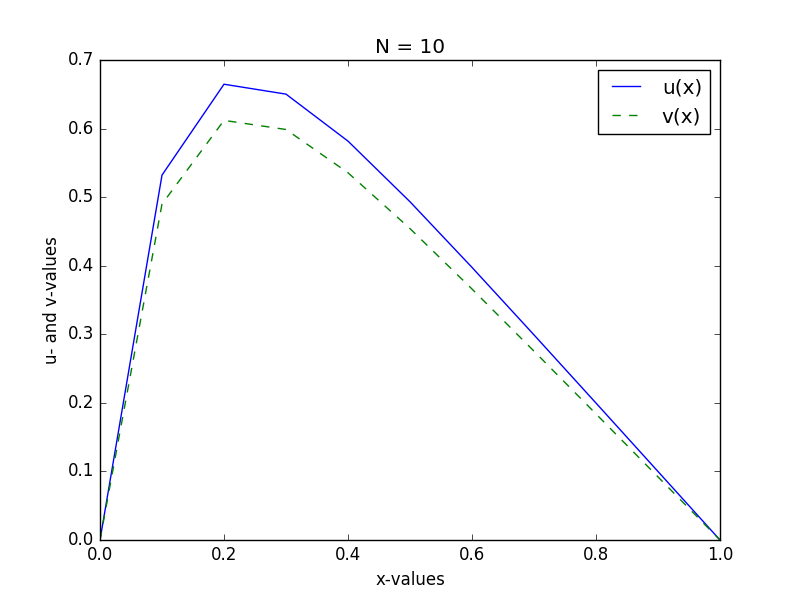
\includegraphics[scale=0.5]{../plots/task_b_N_10.png}
\caption{Our first plot where we have N = 10 points. u(x) is the correct solution and v(x) is the approximated. As we can see that they almost align, but not quite. Especially in the top around x = 0.2.}
\label{fig:N10}
\end{figure}
Afterwards we set the N-value to 100 and got 100 points. The result of this can be seen in \ref{fig:N100S}. As we can see from \ref{fig:N100} and \ref{fig:N100Zoom} we have to zoom in to see any difference. We also ploted for higher values of N, but the results vere much the same as for N = 100 only we had to zoom in even more to see the difference.
\begin{figure}[H]
\centering
\begin{subfigure}{0.3\textwidth}
	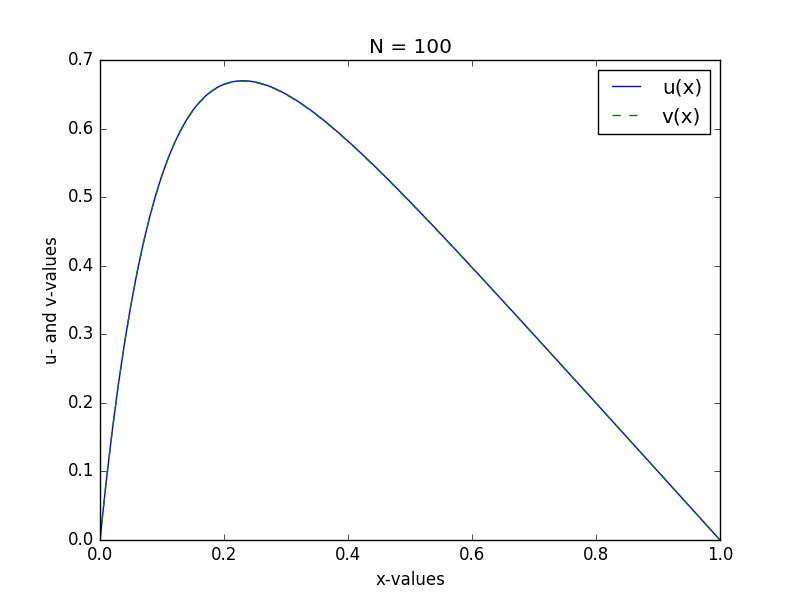
\includegraphics[scale=0.35]{../plots/task_b_N_100.png}
	\caption{The N = 100 case}	
	\label{fig:N100}
\end{subfigure}
\qquad \qquad \qquad
\begin{subfigure}{0.3\textwidth}
	\includegraphics[scale=0.35]{../plots/task_b_N_10zoom.png}
	\caption{The N = 100 case, zoomed in.}
	\label{fig:N100Zoom}
\end{subfigure}
\caption{The plot for N = 100. u(x) and v(x) are the same as above. As we can see the graphs are much more aligned now. On the left we have zoomed in on the top to show the small differences.}
\label{fig:N100S}
\end{figure}
To see the effectiveness of our specialized algorithm we took the time of the general,the specialized algorithm and the LU-decompositionmethod. The result is presented in table \ref{tab:time}.
\begin{table}[H]
\centering
\begin{tabular}{|c|c|c|c|} \hline
$\log_{10}(n)$ & General [sec] & Specialized [sec] & LU-decomposition [sec] \\ \hline
1 &  $2.0\E{-6}$ & $1.0\E{-6}$ & $8.0\E{-6}$ \\ \hline
2 &  $4.0\E{-6}$ & $2.0\E{-6}$ & $4.3\E{-3}$ \\ \hline
3 &  $5.3\E{-5}$ & $2.7\E{-5}$ & $2.2$ \\ \hline
4 &  $6.0\E{-4}$ & $4.2\E{-4}$ & - \\ \hline
5 &  $3.8\E{-3}$ & $2.2\E{-3}$ & - \\ \hline
6 &  $4.2\E{-2}$ & $2.4\E{-2}$ & - \\ \hline
7 &  $0.43$       & $0.26$     & - \\ \hline
\end{tabular}
\caption{This table shows us the time used by the program for different N-values. The last column contains only 3 values because for N = 10000 and above the calculations took too long.}
\label{tab:time}
\end{table}
Lastly we found the relative error using \eqref{eq:error} and the result is presented in \ref{tab:error}.
\begin{table}[H]
\centering
\begin{tabular}{|c|c|} \hline
$log_{10}(h)$ & Relative error \\ \hline
-1 & -1.1 \\ \hline
-2 & -3.1 \\ \hline
-3 & -5.1 \\ \hline
-4 & -7.1 \\ \hline
-5 & -9.0 \\ \hline
-6 & -6.8 \\ \hline
-7 & -13.5  \\ \hline
\end{tabular}
\caption{The relative error between our approximation and the exact solution as a function of step length h.}
\label{tab:error}
\end{table}
\subsection*{Discussion}
Comparing our three methods we can see that the specialized algorithm is superior when it comes to time usage. From table \ref{tab:time} we can see  that there is about a factor of two between the general and the specialized algorithm. This fits our estimation of respectivevly 9n and 4n FLOPS. We can also see that the LU-decomposition is clearly inferior. This is becuase the technique calculates with a whole matrix, while our method with forward and backward substitution only uses the three diagonals that have any value other than zero in them. In our case with such small N-values one can debate if it really was necessary to make a specialized algorithm when the general method only used 0.43 seconds with $n = 10^7$. It is a fair point, however, if we had continued with higher values of n until the program used about half an hour completing the task, I would prefere the method that only used 15 minutes. With this argument we meet another problem. If we continued to high enough values of n, we would have overflow and then the program would not work even if it only used half the time to do it.  \\ 
If i had done this assignment again or need the program in the future, I would want to look over it with fresh eyes and try to make it more effective. I would have liked to find another way or library to do the LU-decomposition. Even if it can't be as effective in the tridiagonal case, it is always useful to have a good way to manipulate whole matrixes at once. \\ \\
From figures \ref{fig:N10} and \ref{fig:N100S} we can clearly see that, for these small values, increasing n will give a better approximation. This is also confirmed by \ref{tab:error} which shows us that the relative error decreases until we have $\log_{10}(h) = -5$. After that it becomes more and then it is smaller again. Why we have this sudden peak at $\log_{10}(h) = -6$ is unclear to me. It may be round of errors or it may be that this exact number of steps gives an uncertainty not present elsewhere. If we increase the step length even further we can see that for $\log_{10}(h) = -8$, we have a relative error at about -2, going higher than that makes my computer crash. This could mean two things: Either we have an anomaly at $\log_{10}(h) = -6$ and the relative error should be lower or at $\log_{10}(h) = -8$ and the relative error should be higher. It would be natural to assume that $\log_{10}(h) = -5$ is the optimal and that afterwards the relative error becomes worse and worse. If I were to do the project again, I would look more into this and run the program for smaller step lengths on a computer with more RAM.
\subsection*{Conclusion}
At the end of the day it is clear to us that the specialized algorithm uses the shortest time and is thus the optimal way to solve this specific task. The approximation becomes better and better until we reach step lengths as small as $\log_{10}(h) = -5$. Even though $\log_{10}(h) = -8$ gives a better relative error, this could be because of something wrong in the program and should be double checked before it is trusted. The LU-decompostion is a slow method because it uses the whole matrix and does not take advantage of the properties of a tridiagonal matrix.
\end{document}